%!TEX root = ../dissertation.tex
\chapter{Supplementary Materials}
\label{app}

\section{Two reuse schemes}
\label{app:2schemes}

The two schemes for reuse described in Figure \ref{fig:changeN}, \emph{summary-based} and \emph{sample-based} amortization, are described below in greater detail. 


In \emph{sample-based amortization}, we simply add samples generated in response to one query ($\mathcal{Q}1$) to the sample set for another query ($\mathcal{Q}2$). So if $N_1$ samples were generated in response to $\mathcal{Q}1$, and $N_2$ new samples are generated in response to $\mathcal{Q}2$, in the absence of amortization, the responses to the two queries $\mathcal{Q}1$ and $\mathcal{Q}2$ would be generated as follows:

\begin{align*}
\textstyle
P(h_{\mathcal{Q}1}|d) & \approx \frac{1}{N_1}\sum_{n=1}^{N_1} \mathbb{I}[h_n=h_{\mathcal{Q}1}]\\
P(h_{\mathcal{Q}2}|d) & \approx \frac{1}{N_2}\sum_{n=1}^{N_2} \mathbb{I}[h_n=h_{\mathcal{Q}2}]\\
\end{align*}

Under the sample-based amortization scheme, the response to $\mathcal{Q}2$ is given by a calculation carried out over all $N_1 + N_2$ equally weighted samples.

\begin{align*}
\textstyle
P(h_{\mathcal{Q}1}|d) & \approx \frac{1}{N_1}\sum_{n=1}^{N_1} \mathbb{I}[h_n=h_{\mathcal{Q}1}]\\
P(h_{\mathcal{Q}2}|d) & \approx \frac{1}{N_2 + N_1}  \left( \sum_{n=1}^{N_1} \mathbb{I}[h_n=h_{\mathcal{Q}2}] + \sum_{n=1}^{N_2} \mathbb{I}[h_n=h_{\mathcal{Q}2}] \right)\\
\end{align*}

Under this scheme, all the computations carried out for $\mathcal{Q}1$ are available for flexible reuse in the computation for $\mathcal{Q}2$. 

In \emph{summary-based amortization}, we reuse a summary statistic computed from $\mathcal{Q}1$. This strategy is only applicable to problems where the answer to $\mathcal{Q}2$ can be expressed as the composition of the answer to $\mathcal{Q}1$, and an additional simpler computation. For example if $\mathcal{Q}1$ is ``What is the probability that there is an object starting with a C in the scene?'', $\mathcal{Q}2$ could be ``What is the probability that there is an object starting with a C or an R in the scene?''. In this case, the $N_1$ samples generated in response to $\mathcal{Q}1$ are summarized into one probability (``the probability of an object starting with C''), $N_2$ new samples are generated in response to a simpler query (``the probability of an object starting with R''), and these two numbers are then composed (in this case simply added) to give the final estimate for $\mathcal{Q}2$ (``the probability of an object starting with C or R''). 


\begin{align*}
\textstyle
P(h_{\mathcal{Q}1}|d) & \approx \frac{1}{N_1}\sum_{n=1}^{N_1} \mathbb{I}[h_n=h_{\mathcal{Q}1}]\\
P(h_{\mathcal{Q}2}|d) & \approx \frac{1}{N_1}\sum_{n=1}^{N_1} \mathbb{I}[h_n=h_{\mathcal{Q}1}] + \frac{1}{N_2}\sum_{n=1}^{N_2} \mathbb{I}[h_n= (h_{\mathcal{Q}2} - h_{\mathcal{Q}1})]\\
\end{align*}


Under this scheme, only the final product of the computation carried out for $\mathcal{Q}1$ is reused in the calculations for $\mathcal{Q}2$.

\newpage

\section{Recognition network architecture}
\label{app:LTI_arch}

We used a three-layer neural network architecture as the function approximator for the approximate posterior. Each unit took as input a linear combination of all the units in the layer below, and then passed this linear combination through a nonlinear transfer function. The details of this architecture varied depending on the structure of the inference problem. 

When the hypothesis space was binary, the output of the network was a Bernoulli parameter; thus, the network implemented a function $f_\phi: \mathcal{D} \mapsto [0,1]$, where $\mathcal{D}$ denotes the data space, and the variational approximation was $Q_\phi(h|d) = \text{Bernoulli}(h; f_\phi(d))$. The data space was modeled by 5 input variables: one for the prior parameter, two for the likelihood parameters, and two for the strength and weight of the evidence, and the output space consisted of a single output that represented a Bernoulli parameter. The hidden units use a radial basis function non-linearity, the mean and variance of which were also optimized, and the activation function at the topmost layer was a softmax in order to ensure the final output lay between 0 and 1. To vary the capacity of the network, we vary the number of hidden units; unless otherwise mentioned, networks contain 1 hidden unit since that provides the strongest bottleneck and best demonstrates the effects of interest. We use 2 hidden units only in the replication of the empirical evidence reviewed in \citet{benjamin18}. Some of the experiments therein are more complex (larger and more varied space of priors, likelihoods and sample sizes) than the subsequent experiments we model, and we found that while a network with 1 hidden unit still captured the qualitative patterns of interest in the empirical results, it could not capture some of the variation and therefore looked visually less similar to the empirical data. We also use a variant of this function approximation architecture in the section on memory-modulated subadditivity, where the number of inputs increases to 12, and the output is a multinomial distribution of dimension 12. 
% In this experiment, the predictions do not hinge on an information bottleneck, and rather on the learned representation of posteriors across queries. 
Learning a 12 dimensional multinomial is much harder than learning a binomial, so we increase the number of hidden units to 10.

When the hypothesis space was real-valued, the output was a mean and log standard deviation parametrizing a Gaussian distribution; thus, the network implemented a function $f_\phi: \mathcal{D} \mapsto \mathbb{R}^2$, and the variational approximation was $Q_\phi(h|d) = \mathcal{N}(h; f_\phi(d))$. The data space was modeled by three inputs: the prior mean, the mean of the evidence and the number of samples, the output space consisted of two outputs that represented the mean and variance of a normal distribution. The hidden units used a hyperbolic tangent activation function, and the activation function at the topmost layer made no transformation at the node representing the mean, and took an exponential at the node representing the variance to ensure that the final output was greater than zero.

\newpage 


\section{Hierarchical Bayesian model in the continuous domain}
\label{app:LTI_HBM}

Here we discuss the predictions of a hierarchical Bayesian model that learns about the underlying global variances from experience. We refer to it henceforth as the L-HBM, for learned hierarchical Bayesian model. We find that it cannot reproduce the observed effect of differentially strong reactions to data between the high and the low dispersion condition. 

The L-HBM assumes the true generative model described in the section `Extension to a continuous domain'. The output $y_{kn}$ for trial $n$ in a block $k$ is drawn from $\mathcal{N}(m_k,s)$. These $m_k$ values are distributed over blocks as $\mathcal{N}(m_0,v)$.


\begin{figure}[hb!]
\centering
    \includegraphics[width=0.5\textwidth]{figures/samstan.pdf}
  \caption{\textbf{Performance of the L-HBM}. Simulation results of a hierarchical Bayesian model that infers the underlying parameters in the the experiment reported by \cite{gershman2017blessing}. The Y-axis shows the L-HBM's updates from prior to posterior ($\Delta$Data) and the X-axis shows the update of a rational (hierarchical) model ($\Delta$Rational; a HBM that knows the true parameters for the underlying generative process). Error bars represent the standard error of the mean. Gray line represents $y=x$.} 
  \label{fig:App:hierBayes}
\end{figure}

The true values of these parameters are as follows: $s = 25, m_0 = 40$ for all participants. In the high dispersion condition $v = 144$ and in the low dispersion condition $v = 36$.  The HBM discussed in the main text receives these correct values for the parameters. The L-HBM discussed here has to infer these values. The prior distributions we assume for $m_0$, $s$, and $v$ in the L-HBM are $\mathcal{N}(40,10)$, half-$\mathrm{Cauchy}(0,10)$, and half-$\mathrm{Cauchy}(0,10)$, respectively. It then receives the observations $y_{kn}$ and can form a joint posterior distribution over $m_0$, $s$, and $v$. With these it can then form a posterior predictive distribution for $m_k$ in that block, which we use as the predicted output on each trial.

% where $\mu$ is the average output over all options, and $\tau^2$ the variance of the button-specific means. Having observed outputs of the buttons, the model updates these to a joint posterior distribution over the means $\mu_j$, the common mean $\mu$, and the variances $\sigma^2$ and $\tau^2$. At any time $t$, the joint posterior distribution provides posterior predictive distributions of the average output for each button, which we use to make predictions for the output on each trial. We simulate the output of this model using the exact same set-up as was used for our Learned Inference Model previously. 

We compared the resulting updates of this L-HBM to the updates from the HBM in the main text that knows the true parameters of the underlying generative distributions (see Fig.~\ref{fig:App:hierBayes}). For both the high and the low dispersion conditions, the updates closely follow the diagonal line of $y=x$. This indicates that inferring $m_0$, $s$, and $v$ (in addition to $m_k$) does not result in significant differences in the updates in an ideal observer. Crucially, the L-HBM does not replicate the main qualitative effect of a significant difference in updates between the high and the low dispersion condition, for the same rational update. This means that---unlike our Learned Inference Model---a hierarchical Bayesian model cannot reproduce the qualitative effects observed in the experiment.

\newpage

\section{Causal Bayes Nets}
\label{app:causal_cbn}

By combining graph theory and probability theory, the causal Bayesian network framework provides us with a graphical tool to formalize and test different levels of causal reasoning. This section introduces the main definitions underlying this framework and explains how to visually test for statistical independence  \citep{pearl88probabilistic,bishop06pattern,kollerl09probabilistic,barber12bayesian,murphy12machine}.


A {\bf graph} is a collection of nodes and links connecting pairs of nodes.
The links may be directed or undirected, giving rise to {\bf directed} or {\bf undirected graphs} respectively.\\[5pt]
A {\bf path} from node $X_i$ to node $X_j$ is a sequence of linked nodes starting
at $X_i$ and ending at $X_j$. A {\bf directed path} is a path whose links are directed and pointing from preceding towards following nodes in the sequence.\\[5pt]
%\jane{add def CBN here}

\begin{wrapfigure}{l}{0.5\textwidth}
\centering
\subfloat[]{\scalebox{0.7}{
\begin{tikzpicture}[dgraph]
\node[ocont] (x2) at (4.5,0) {$X_2$};
\node[ocont] (x1) at (1.5,0) {$X_1$};
\node[ocont] (x3) at (3,0) {$X_3$};
\node[ocont] (x4) at (3,-1.5) {$X_4$};
\draw[line width=1.15pt](x1)--(x3);\draw[line width=1.15pt](x2)--(x3);\draw[line width=1.15pt](x3)--(x4);\draw[line width=1.15pt](x2)to [bend left=35](x4);
\end{tikzpicture}}}
\hskip0.2cm
\subfloat[]{\scalebox{0.7}{
\begin{tikzpicture}[dgraph]
\node[ocont] (x2) at (4.5,0) {$X_2$};
\node[ocont] (x1) at (1.5,0) {$X_1$};
\node[ocont] (x3) at (3,0) {$X_3$};
\node[ocont] (x4) at (3,-1.5) {$X_4$};
\draw[line width=1.15pt](x1)--(x3);\draw[line width=1.15pt](x2)--(x3);\draw[line width=1.15pt](x3)--(x4);\draw[line width=1.15pt](x2)to [bend left=35](x4);\draw[line width=1.15pt](x4)to [bend left=35](x1);
\end{tikzpicture}}}
% \vspace{-0.15cm}
\caption{(a): Directed acyclic graph. The node $X_3$ is a collider on the path $X_1 \rightarrow X_3 \leftarrow X_2$ and a non-collider on the path $X_2\rightarrow X_3\rightarrow X_4$. (b): Cyclic graph obtained from (a) by adding a link from $X_4$ to $X_1$.}
\label{fig:indep_HMM}
\vspace{-0.75cm}
\end{wrapfigure}A {\bf directed acyclic graph} is a directed graph with no
directed paths starting and ending at the same node. For example, the directed graph in Figure \ref{fig:indep_HMM}(a) is acyclic. 
The addition of a link from $X_4$ to $X_1$ gives rise to a cyclic graph (Figure \ref{fig:indep_HMM}(b)).\\[5pt]
A node $X_i$ with a directed link to $X_j$ is called {\bf parent}
of $X_j$. In this case, $X_j$ is called {\bf child} of $X_i$.\\[5pt]
A node is a {\bf collider} on a specified path if it has (at least) two parents on that path.
Notice that a node can be a collider on a path and a non-collider on another path. For example, in Figure \ref{fig:indep_HMM}(a) $X_3$ is a collider on the path $X_1 \rightarrow X_3 \leftarrow X_2$ and a non-collider on the path $X_2\rightarrow X_3\rightarrow X_4$.\\[5pt]
A node $X_i$ is an {\bf ancestor} of a node $X_j$ if there exists a directed path from $X_i$ to $X_j$. In this case, $X_j$ is a {\bf descendant} of $X_i$.\\[5pt]
A {\bf graphical model} is a graph in which nodes represent random variables and links express statistical relationships between the variables.\\[5pt]
A {\bf Bayesian network} is a directed acyclic graphical model in which each node $X_i$ is associated
with the conditional distribution $p(X_i|\text{pa}(X_i))$, where $\text{pa}(X_i)$ indicates the parents of $X_i$. The joint distribution of all nodes in
the graph, $p(X_{1:N})$, is given by the product of all conditional distributions, i.e. $p(X_{1:N})=\prod_{i=1}^Np(X_i|\text{pa}(X_i))$.

When equipped with causal semantic, namely when describing the process underlying the data generation, a Bayesian network expresses both causal and statistical relationships among random variables---in such a case the network is called {\bf causal}.  

\paragraph{Assessing statistical independence in Bayesian networks.}
Given the sets of random variables ${\cal X}, {\cal Y}$ and ${\cal Z}$,
${\cal X}$ and ${\cal Y}$ are statistically independent given ${\cal Z}$ if all paths
from any element of ${\cal X}$ to any element of ${\cal Y}$ are {\bf closed} (or {\bf blocked}). A path is closed if at least one of the following conditions is satisfied:
\begin{enumerate}
\setlength{\itemsep}{-2pt}  
%\setlength{\parskip}{-4pt}
\setlength{\parsep}{-4pt}
\item[(i)] There is a non-collider on the path which belongs to the conditioning set ${\cal Z}$.
\item[(ii)] There is a collider on the path such that neither the collider nor any of its descendants belong to ${\cal Z}$.
\end{enumerate}

\section{Scaling up causal experiments}
\label{app:causal_addexpt}

The purview of the experiments in the main text was to show a proof of concept on a simple tractable system, demonstrating that causal induction and inference can be learned and implemented via a meta-learned agent. In the following, we scale up our results to more complex systems in two new experiments.

\subsection{Experiment 4: Non-linear Causal Graphs}

\begin{figure}[ht!]
\centering
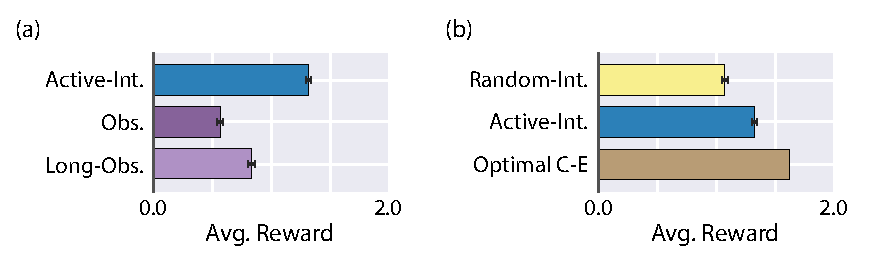
\includegraphics[width=0.7\textwidth]{figures/Nonlinear_results.pdf} 
\caption{Results for non-linear graphs. (a) Comparing average episode reward for agents trained with different data. (b) Comparing information phase intervention policies. }
\label{fig:nonlinear_results}
% \vspace{-0.3cm}
\end{figure}

In this experiment, we generalize some of our results to nonlinear, non-Gaussian causal graphs which are more typical of real-world causal graphs and to demonstrate that our results hold without loss of generality on such systems. 

Here we investigate causal Bayesian networks (\CBNs) with a quadratic dependence on the parents by changing the conditional distribution to $p(X_{i}|\textrm{pa}(X_{i})) = \mathcal{N}(\frac{1}{N_{i}} \sum_{j} w_{ji}(X_{j} + X_{j}^2), \sigma)$. Here, although each node is normally distributed given its parents, the joint distribution is not multivariate Gaussian due to the non-linearity in how the means are determined. We find that the Long-Observational Agent achieves more reward than the Observational Agent indicating that the agent is in fact learning the statistical dependencies between the nodes, within an episode.
\footnote{The conditional distribution $p(X_{1:N\setminus j }|X_j=5)$, and therefore Conditional Agents, were non-trivial to calculate for the quadratic case, and was thus omitted.}
We also find that the Active-Interventional Agent achieves reward well above the best agent with access to only observational data (Long-Observational in this case) indicating an ability to reason from interventions. We also see that the Active-Interventional Agent performs better than the Random-Interventional Agent, indicating an ability to choose informative interventions.


\subsection{Experiment 5: Larger Causal Graphs}

\begin{figure}[ht!]
\centering
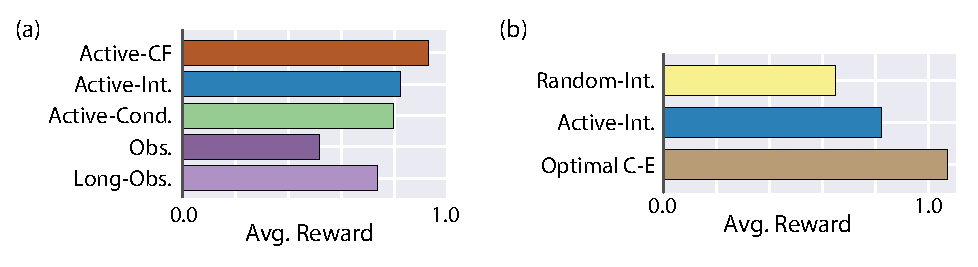
\includegraphics[width=0.7\textwidth]{figures/N6_results_active.pdf} 
\caption{Results for $N=6$ graphs. (a) Comparing average episode reward for agents trained with different data. (b) Comparing information phase intervention policies. }
\label{fig:N6_results}
% \vspace{-0.3cm}
\end{figure}
In this experiment we scaled up to larger graphs with $N=6$ nodes, which afforded considerably more unique \CBNs~than with $N=5$ ($1.4\times10^7$ vs $5.9\times10^4$). As shown in Figure \ref{fig:N6_results}a, we find the same pattern of behavior noted in the main text where the rewards earned are ordered such that Observational agent $<$ Active-Conditional agent $<$ Active-Interventional agent $<$ Active-Counterfactual agent. We see additionally in Figure \ref{fig:N6_results}b that the Active-Interventional agent performs significantly better than the baseline Random-Interventional agent, indicating an ability to choose non-random, informative interventions.

\newpage


